\documentclass{standalone}
  \usepackage{tikz}
  \usetikzlibrary{arrows, automata, positioning}
  \tikzstyle{automaton}=[shorten >=1pt, pos=.4,
                         >=stealth', initial text=]
  \tikzstyle{accepting}=[accepting by arrow]

\begin{document}
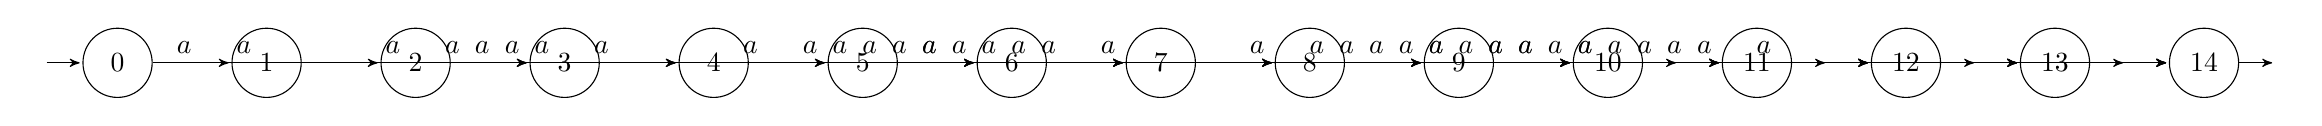
\begin{tikzpicture}[automaton]
  \node[state,initial] (0) {$0$};
  \node[state] (1) [right=of 0] {$1$};
  \node[state] (2) [right=of 1] {$2$};
  \node[state] (3) [right=of 2] {$3$};
  \node[state] (4) [right=of 3] {$4$};
  \node[state] (5) [right=of 4] {$5$};
  \node[state] (6) [right=of 5] {$6$};
  \node[state] (7) [right=of 6] {$7$};
  \node[state] (8) [right=of 7] {$8$};
  \node[state] (9) [right=of 8] {$9$};
  \node[state,accepting] (10) [right=of 9] {$10$};
  \node[state,accepting] (11) [right=of 10] {$11$};
  \node[state,accepting] (12) [right=of 11] {$12$};
  \node[state,accepting] (13) [right=of 12] {$13$};
  \node[state,accepting] (14) [right=of 13] {$14$};
  \path[->] (0) edge node[above] {$a$} (1);
  \path[->] (0) edge node[above] {$a$} (2);
  \path[->] (1) edge node[above] {$a$} (3);
  \path[->] (1) edge node[above] {$a$} (4);
  \path[->] (1) edge node[above] {$a$} (5);
  \path[->] (2) edge node[above] {$a$} (3);
  \path[->] (2) edge node[above] {$a$} (4);
  \path[->] (2) edge node[above] {$a$} (5);
  \path[->] (3) edge node[above] {$a$} (6);
  \path[->] (3) edge node[above] {$a$} (7);
  \path[->] (3) edge node[above] {$a$} (8);
  \path[->] (3) edge node[above] {$a$} (9);
  \path[->] (4) edge node[above] {$a$} (6);
  \path[->] (4) edge node[above] {$a$} (7);
  \path[->] (4) edge node[above] {$a$} (8);
  \path[->] (4) edge node[above] {$a$} (9);
  \path[->] (5) edge node[above] {$a$} (6);
  \path[->] (5) edge node[above] {$a$} (7);
  \path[->] (5) edge node[above] {$a$} (8);
  \path[->] (5) edge node[above] {$a$} (9);
  \path[->] (6) edge node[above] {$a$} (10);
  \path[->] (6) edge node[above] {$a$} (11);
  \path[->] (6) edge node[above] {$a$} (12);
  \path[->] (6) edge node[above] {$a$} (13);
  \path[->] (6) edge node[above] {$a$} (14);
  \path[->] (7) edge node[above] {$a$} (10);
  \path[->] (7) edge node[above] {$a$} (11);
  \path[->] (7) edge node[above] {$a$} (12);
  \path[->] (7) edge node[above] {$a$} (13);
  \path[->] (7) edge node[above] {$a$} (14);
  \path[->] (8) edge node[above] {$a$} (10);
  \path[->] (8) edge node[above] {$a$} (11);
  \path[->] (8) edge node[above] {$a$} (12);
  \path[->] (8) edge node[above] {$a$} (13);
  \path[->] (8) edge node[above] {$a$} (14);
  \path[->] (9) edge node[above] {$a$} (10);
  \path[->] (9) edge node[above] {$a$} (11);
  \path[->] (9) edge node[above] {$a$} (12);
  \path[->] (9) edge node[above] {$a$} (13);
  \path[->] (9) edge node[above] {$a$} (14);
\end{tikzpicture}
\end{document}
